% Replace the internal-routing portion of experimental_diagnostics.tex.
% The former fusion identities and Square diagnostics must be included
% only in the routing/fusion appendix, not repeated here.
% Existing labels are retained for compatibility. Requires amsmath,
% booktabs, and graphicx; reuses the two original routing PDFs.

\section{Internal expert routing: protocols and supplementary results}
\label{app:routing_physics}

\subsection{Circular: internal expert utilization}
\label{app:internal_routing}

This study characterizes correction-expert selection and weight allocation
inside individual regime-local specialists, rather than E2 selection
between specialists. We first define the sampling protocol and metrics,
then distinguish aggregate utilization, parameter-dependent allocation,
and variation along autonomous rollouts. The results describe the
evaluated checkpoints and windows, not all trained configurations.

\paragraph{Checkpoints and sampling protocol.}
We analyze frozen original Circular Hopf and Periodic specialists,
not the repaired three-seed models. Periodic is evaluated on 13 fixed
windows at each of four held-out Reynolds numbers, giving 52 windows
with $K=48$. Hopf uses five windows at each of three held-out Reynolds
numbers, giving 15 windows with $K=56$. These differ from the controlled
local reevaluation in Appendix~\ref{app:circular}.
We record one routing decision per output step at the first integration
stage, giving 2496 Periodic and 840 Hopf records per channel, rather
than counting every intermediate right-hand-side evaluation.
The statistics pool these records; overlapping windows are not treated
as independent trajectories. No routing diagnostic is used for
checkpoint selection.

\paragraph{Selection frequency and mixing weight.}
For each channel, let $I_{n,e}$ indicate whether routed expert $e$ is
selected at record $n$, including group identity in the expert index.
For $N$ records, define
\begin{equation}
f_e=\frac{1}{2N}\sum_{n=1}^{N}I_{n,e},
\qquad \sum_e f_e=1,
\label{eq:app_routing_frequency}
\end{equation}
where the factor two accounts for Top-2 activation at each record.
This is the fraction of selected expert slots, not the fraction of
time steps at which an expert is active. The mean routing mass is
\begin{equation}
m_e=\frac{1}{N}\sum_{n=1}^{N}\omega_{n,e}I_{n,e},
\label{eq:app_routing_mass}
\end{equation}
where $\omega_{n,e}$ is the final mixing coefficient, including the
scaling of the routed component. Unselected experts retain zero
frequency and mass. For these two checkpoints, the shared component
has coefficient $4/7$ and the routed Top-2 component has total
coefficient $3/7$, so $\sum_e m_e=3/7$.
The shared expert is excluded from the routed-expert counts below.
Routing mass quantifies weight allocation, not expert-output magnitude;
an expert's weight is not itself a measure of its physical contribution.
Identifiers such as \texttt{g0:e0} are local routed-expert labels and
do not denote the shared expert.

\paragraph{Selection diversity.}
With $N_E$ routed experts available to a channel, define
\begin{equation}
H=-\frac{\sum_{e:f_e>0}f_e\log f_e}{\log N_E},
\qquad 0\leq H\leq1.
\label{eq:app_routing_entropy}
\end{equation}
This entropy measures dispersion of activation frequencies, not mixing
weights or temporal switching. We also count distinct unordered Top-2
pairs, retaining group identity, and the fraction of records assigned
to the most frequent pair. An expert is counted as active if selected
at least once in the evaluated records.

\begin{table}[tbp]
\centering\small
\setlength{\tabcolsep}{5pt}
\caption{Post-hoc Circular internal-routing statistics. Active experts
are reported relative to all available routed experts; the shared
expert is excluded. Pair counts retain group identity. Dominant-pair
share is the fraction of records using the most frequent unordered
pair, and $H$ is activation-frequency entropy.}
\label{tab:internal_routing_summary}
\begin{tabular}{@{}llrrrr@{}}
\toprule
Specialist & Channel & \shortstack{Active\\experts}
& \shortstack{Distinct\\Top-2 pairs}
& \shortstack{Dominant-pair\\share (\%)} & $H$\\
\midrule
Hopf & Velocity & 2/6 & 1 & 100.00 & 0.387\\
& Pressure & 2/6 & 1 & 100.00 & 0.387\\
\addlinespace
Periodic & Velocity & 18/18 & 33 & 16.27 & 0.929\\
& Pressure & 14/18 & 16 & 31.25 & 0.784\\
\bottomrule
\end{tabular}
\end{table}

\paragraph{Periodic: broad but channel-dependent utilization.}
Table~\ref{tab:internal_routing_summary} shows that Periodic activates
all available velocity experts and most pressure experts. Velocity
selection is more dispersed than pressure selection, with more distinct
pairs, a smaller dominant-pair share, and higher utilization entropy.
Figure~\ref{fig:periodic_internal_routing} separates group frequencies
from routed-expert masses across the four held-out Reynolds numbers.
The group-selection frequencies vary across parameters, while the
channel-specific masses reveal how the routed weight is distributed.
These are utilization patterns, not assignments of physical mechanisms
to individual experts.

\paragraph{Hopf: fixed support with nonuniform weights.}
Hopf has a single group by architecture; the absence of group switching
is therefore not evidence that a learned multi-group router has collapsed.
Within that group, the observed velocity pair is $(e_1,e_3)$ and the
pressure pair is $(e_2,e_4)$ at every recorded step. Unlike the single-group
architecture, this fixed pair selection is an empirical observation on
the evaluated windows. A separate stage-wise check also found the same
pairs across all four Runge--Kutta stages.

Velocity expert $e_3$ receives approximately $99.93\%$ of the routed
mass, and pressure expert $e_2$ receives $84.16\%$. These percentages
are relative to the routed component, not the complete correction
including the shared expert. The secondary pressure expert $e_4$
has a mean mass that increases across the three evaluated Reynolds
numbers, so fixed support does not imply constant weight allocation.
For a fixed pair, both activation frequencies equal $1/2$ and
$H=\log 2/\log 6\simeq0.387$, regardless of how uneven their weights
are. Thus the entropy in the table does not indicate pair switching
or balanced expert contributions.

\paragraph{Allocation along Periodic rollouts.}
Figure~\ref{fig:periodic_routing_step} reports the mean routed-expert
mass at each normalized prediction position $k/48$, averaging the same
52 windows. It complements the parameter-wise statistics by showing
allocation along the autonomous rollout. Since the windows are not
aligned by physical oscillation phase, these profiles cannot establish
phase-specific expert specialization. Nor do aggregate utilization
statistics establish a causal accuracy benefit; that question requires
the controlled prediction comparisons rather than expert counts alone.

\begin{figure}[tbp]
\centering
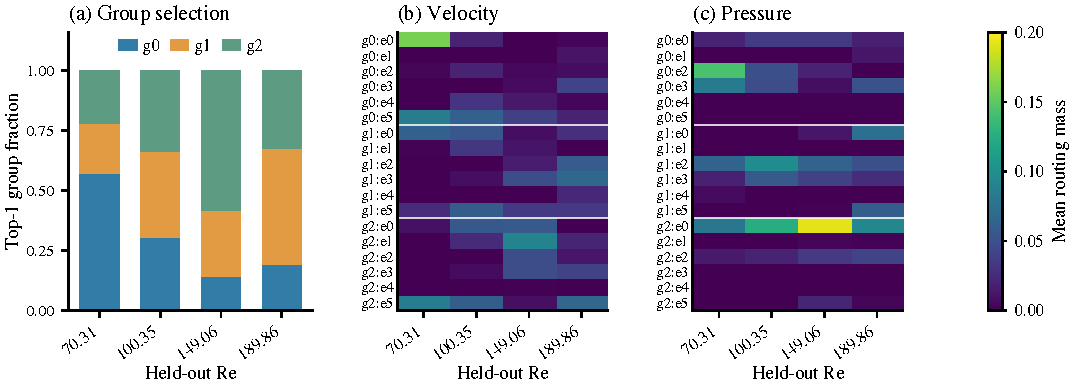
\includegraphics[width=\linewidth]{figures/periodic_internal_routing.pdf}
\caption{Parameter-dependent internal routing of the frozen Circular
Periodic specialist. (a) Top-1 group-selection frequencies.
(b,c) Mean routed-expert mass for velocity and pressure, respectively.
Records are collected at the first integration stage of each output
step over 13 windows per Reynolds number. Expert labels are local to
each group and channel; the shared component is not shown.}
\label{fig:periodic_internal_routing}
\end{figure}

\begin{figure}[tbp]
\centering
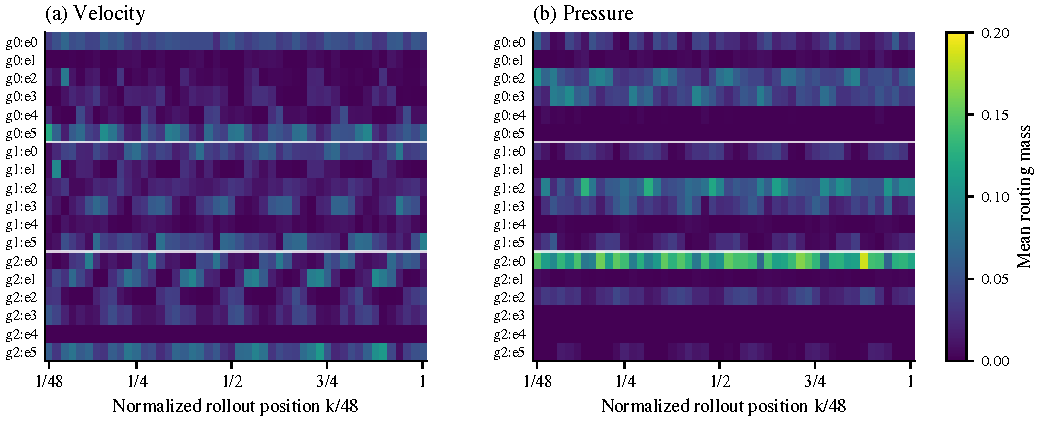
\includegraphics[width=\linewidth]{figures/periodic_rollout_step_routing.pdf}
\caption{Periodic routed-expert mass along autonomous rollouts.
Each column averages records at the same output step across 52 windows;
all routed experts are retained. The horizontal coordinate $k/48$
denotes normalized prediction position, not physical oscillation phase.
Masses include the routed-component scaling and exclude the shared
expert.}
\label{fig:periodic_routing_step}
\end{figure}
